\documentclass[11pt,a4paper]{article}
\usepackage[margin=2.4cm]{geometry}
\usepackage{amsmath,amssymb,amsthm}
\usepackage{graphicx}
\usepackage{booktabs}
\usepackage{array}
\usepackage[font=small,labelfont=bf,labelsep=period]{caption}
\usepackage{wrapfig}
\usepackage{microtype}
\usepackage[hidelinks]{hyperref}
\usepackage{xurl}

\newtheorem{theorem}{Theorem}
\newtheorem{lemma}{Lemma}
\newcommand{\R}{\mathbb R}
\newcommand{\Z}{\mathbb Z}
\DeclareMathOperator{\diam}{diam}
\newcommand{\repo}{https://github.com/Sager611/riemann/blob/main/}
\newcommand{\lean}[2]{\href{\repo #2}{\texttt{#1}}}
\newcommand{\RB}{\mathcal A}
\newcommand{\CB}{\mathcal B}
\setlength{\abovecaptionskip}{4pt}
\captionsetup[table]{skip=3pt}

\title{Gale's conjecture fails in dimensions 7 and 8,\\ hence in every dimension $n\ge 3$}
\author{\href{https://github.com/Sager611/riemann}{github.com/Sager611/riemann}}
\date{November 2026}

\begin{document}
\maketitle

\begin{abstract}
\noindent Gale (1953) conjectured that the ball is the hardest bounded set in $\R^n$ to split into $n+1$ parts of small diameter. Counterexamples were known for $n=3,\dots,6$ and $n\ge 9$. We give finite counterexamples in $\R^7$ (84 points) and $\R^8$ (85 points), and a family, built from two regular simplices in orthogonal subspaces, that is a counterexample in every dimension $5\le n\le 1000$, with a proof that needs no search over colourings. Hence Gale's conjecture fails in every dimension $n\ge 3$.

\smallskip\noindent\emph{Note.} The results were found and checked with AI agents, with computer certificates and a Lean~4/Mathlib formalization (\S\ref{sec:lean}); this paper has not been peer reviewed.
\end{abstract}

\section{Motivation}

\begin{wrapfigure}{r}{0.25\textwidth}
\vspace{-14pt}
\centering
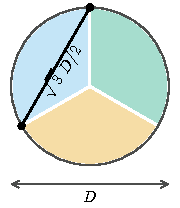
\includegraphics[width=0.22\textwidth]{figs/disk.pdf}
\captionsetup{justification=raggedright,singlelinecheck=false}
\caption{A disk of diameter $D$ cut into three $120^\circ$ sectors, each of diameter $\frac{\sqrt3}{2}D$ (chord). No split into 3 parts does better~\cite{Ga53}.}
\label{fig:disk}
\vspace{-10pt}
\end{wrapfigure}

Borsuk asked in 1933 whether every bounded set in $\R^n$ splits into $n+1$ parts of smaller diameter; the ball shows that $n$ parts are not enough~\cite{Bo33}. Kahn and Kalai showed that the answer is no for large $n$~\cite{KK93}, and Hinrichs for every $n>322$~\cite{Hi02}. The lowest dimension with a known counterexample is 64~\cite{JB14}, or 9 in an unrefereed preprint~\cite{OAI26}.

Gale asked how small the $n+1$ parts can be~\cite{Ga53}. A set of diameter $D$ on a line splits into two parts of diameter at most $D/2$, and a planar set into three parts of diameter at most $\frac{\sqrt3}{2}D$; a segment and a disk (Fig.~\ref{fig:disk}) show that both bounds are sharp~\cite{Ga53}. Gale conjectured that in every dimension the ball is the hardest set to split (\S\ref{sec:def} states this precisely).

Before this paper the conjecture was known to fail for $n=3,\dots,6$, by point sets found by computer search~\cite{Vo26}, and in every dimension in which Borsuk's conjecture fails (\S\ref{sec:all}). Dimensions 7 and 8 were open. Voronov asked for counterexamples in every dimension $n\ge 3$, described geometrically and proved without enumerating graph colourings~\cite{Vo26}.

We give finite counterexamples in $\R^7$ and $\R^8$ (Theorem~\ref{thm:x78}, Fig.~\ref{fig:sets}) and one family that is a counterexample in every dimension $5\le n\le 1000$, with a proof by hand of its combinatorial step (Theorem~\ref{thm:family}); this answers Voronov's question for these $n$. With our earlier sets for $n=3,4$ and Hinrichs's sets for $n>1000$, Gale's conjecture fails in every dimension $n\ge 3$ (Theorem~\ref{thm:main}).

\section{Definitions}\label{sec:def}

For bounded $V\subset\R^n$ and integers $k\ge 1$, with $\|\cdot\|$ the Euclidean norm and $[k]=\{1,\dots,k\}$:
\[
\diam V=\sup_{x,y\in V}\|x-y\|,\qquad
\beta_k(V)=\inf_{\varphi:\,V\to[k]}\ \max_{i\in[k]}\ \diam \varphi^{-1}(i).
\]
A map $\varphi:V\to[k]$ is a \emph{partition} of $V$ into the $k$ parts $\varphi^{-1}(1),\dots,\varphi^{-1}(k)$ (empty parts allowed, $\diam\emptyset=0$); we also call $\varphi$ a \emph{$k$-colouring} and $\varphi(x)$ the \emph{colour} of $x$. So $\beta_k(V)$ is the least possible largest part diameter.

Let $B^n$ be the closed ball of diameter 1 centred at $0$. The cones $\{\lambda y:\lambda\ge0,\ y\in F\}$ over the $n+1$ facets $F$ of a regular simplex inscribed in $B^n$ cut $B^n$ into $n+1$ congruent parts of diameter~\cite[\S1]{Vo26}
\begin{equation}\label{eq:sigma}
\sigma_n=\sqrt{\frac{n+1}{n+2}}\ \ (n\text{ even}),\qquad
\sigma_n=\sqrt{\frac12+\frac12\sqrt{\frac{n-1}{n+3}}}\ \ (n\text{ odd}),\qquad n\ge 2,
\end{equation}
so $\beta_{n+1}(B^n)\le\sigma_n$, with equality for $n=2,3$~\cite{Vo26}. For example $\sigma_2=\frac{\sqrt3}{2}$ (Fig.~\ref{fig:disk}), $\sigma_7=0.9419651451\ldots$ and $\sigma_8=0.9486832980\ldots$

\smallskip
\noindent\textbf{Gale's conjecture in $\R^n$~\cite{Ga53,Vo26}.} Every bounded $V\subset\R^n$ satisfies $\beta_{n+1}(V)\le\beta_{n+1}(B^n)\diam V$.

\smallskip
\noindent A \emph{counterexample} in $\R^n$ is a bounded $V\subset\R^n$ with $\beta_{n+1}(V)>\sigma_n\diam V$. Since $\beta_{n+1}(B^n)\le\sigma_n$, it refutes Gale's conjecture in $\R^n$.

\section{Main result}\label{sec:main}

\begin{theorem}\label{thm:main}
For every $n\ge 3$ there is a counterexample in $\R^n$; for $n\le 1000$ it is an explicit finite set. Hence Gale's conjecture fails in every dimension $n\ge 3$.
\end{theorem}

\begin{table}[h]
\centering\small
\caption{The counterexamples $X$ of Theorem~\ref{thm:main}. All rows with $n\le1000$ are also proved in Lean (\S\ref{sec:lean}).}
\label{tab:main}
\setlength{\tabcolsep}{4pt}
\begin{tabular}{@{}llrlll@{}}
\toprule
$n$ & $X$ & $|X|$ & $\beta_{n+1}(X)/\diam X$ & $\sigma_n$ & certified by\\
\midrule
3 & $X_3$ & 170 & $0.8906210556\ldots$ & $0.8880738339\ldots$ & computer search, \S\ref{sec:all}\\
4 & $X_4$ & 126 & $0.9164673596\ldots$ & $0.9128709291\ldots$ & computer search, \S\ref{sec:all}\\
7 & $X_7$ & 84 & $0.9434435130\ldots$ & $0.9419651451\ldots$ & computer search, \S\ref{sec:sets}\\
8 & $X_8$ & 85 & $0.9499470677\ldots$ & $0.9486832980\ldots$ & colouring lemma, \S\ref{sec:family}\\
$5,\dots,1000$ & $V_n(\theta_n)$ & 43 to 754005 & $>\sigma_n$ & & colouring lemma, \S\ref{sec:family}\\
$>1000$ & Hinrichs's set~\cite{Hi02} & & $1$ & $<1$ & citation, \S\ref{sec:all}\\
\bottomrule
\end{tabular}
\end{table}

\section{A finite criterion}\label{sec:crit}

For finite $X\subset\R^n$ and $s>0$ let $G_{\ge s}(X)$ and $G_{>s}(X)$ be the graphs on the vertex set $X$ in which $x\ne y$ are adjacent when $\|x-y\|\ge s$, respectively $\|x-y\|>s$. A colouring of a graph is \emph{proper} if adjacent vertices get different colours; the \emph{chromatic number} $\chi(G)$ is the least $k$ for which $G$ has a proper $k$-colouring.

\begin{lemma}\label{lem:crit}
Let $X\subset\R^n$ be finite, $k\ge 1$ and $s>0$. Then
\textup{(a)} $\beta_k(X)\ge s\iff\chi(G_{\ge s}(X))>k$, and
\textup{(b)} $\beta_k(X)\le s\iff\chi(G_{>s}(X))\le k$.
\end{lemma}

\begin{proof}
A $k$-colouring $\varphi$ of $X$ has a part of diameter $\ge s$ if and only if two points $x\ne y$ with $\varphi(x)=\varphi(y)$ have $\|x-y\|\ge s$, that is, if and only if $\varphi$ is not proper on $G_{\ge s}(X)$. Applying this to every $\varphi$ gives (a). For (b): $X$ is finite, so the infimum defining $\beta_k(X)$ is attained, and a $\varphi$ whose parts all have diameter $\le s$ is the same as a proper colouring of $G_{>s}(X)$.
\end{proof}

So $\beta_k(X)=s$ has a certificate in two parts: a proof that $G_{\ge s}(X)$ has no proper $k$-colouring, and one proper $k$-colouring of $G_{>s}(X)$. Our sets $X_3$, $X_4$, $X_7$, $X_8$ have coordinates in $10^{-8}\Z$, so every squared distance is an integer multiple of $10^{-16}$. With $D=\diam X$, the inequality $s>\sigma_n D$ is, by~\eqref{eq:sigma}, equivalent to a test on these integers:
\begin{equation}\label{eq:test}
(n+1)D^2<(n+2)s^2\ \ (n\text{ even});\qquad D^2<2s^2\ \text{ and }\ (n-1)D^4<(n+3)(2s^2-D^2)^2\ \ (n\text{ odd}).
\end{equation}

\section{The sets $X_7$ and $X_8$}\label{sec:sets}

Both sets come from one construction. Write $\R^n=\R^{m_1}\oplus\R^{m_2}$ and $x=(x',x'')$, with $m_1=\lfloor n/2\rfloor$, $m_2=\lceil n/2\rceil$. Let $p=m_1+1$, $q=m_2+1$, $I=\{0,\dots,m_1\}$, $J=\{0,\dots,m_2\}$, and fix unit vectors $u_i\in\R^{m_1}$ ($i\in I$) and $v_j\in\R^{m_2}$ ($j\in J$) with
\[
\langle u_i,u_{i'}\rangle=-\tfrac{1}{m_1}\ \ (i\ne i'),\qquad \langle v_j,v_{j'}\rangle=-\tfrac{1}{m_2}\ \ (j\ne j'):
\]
the vertices of two regular simplices centred at $0$. For parameters $\theta=(r_A,r_B,a,b,c,d,e,f)$, all positive, the set $V_n(\theta)$ consists of the following $p+q+3pq$ points of five types.

\begin{table}[h]
\centering\small
\begin{minipage}[t]{0.42\textwidth}\centering
\caption{The points of $V_n(\theta)$, $i\in I$, $j\in J$.}\label{tab:construction}
\begin{tabular}{@{}lccr@{}}
\toprule
point & $x'$ & $x''$ & number\\
\midrule
$P_i$ & $r_A u_i$ & $0$ & $p$\\
$Q_j$ & $0$ & $r_B v_j$ & $q$\\
$A_{ij}$ & $a\,u_i$ & $-b\,v_j$ & $pq$\\
$B_{ij}$ & $-c\,u_i$ & $d\,v_j$ & $pq$\\
$C_{ij}$ & $e\,u_i$ & $f\,v_j$ & $pq$\\
\bottomrule
\end{tabular}
\end{minipage}\hfill
\begin{minipage}[t]{0.53\textwidth}\centering
\caption{The parameters $\theta_7$, $\theta_8$, rounded; exact 12-decimal values in \href{\repo Riemann/Deep/Gale7/family_params.txt}{\texttt{family\_params.txt}}.}\label{tab:params}
\setlength{\tabcolsep}{3.2pt}
\begin{tabular}{@{}lcccccccc@{}}
\toprule
$n$ & $r_A$ & $r_B$ & $a$ & $b$ & $c$ & $d$ & $e$ & $f$\\
\midrule
7 & .6124 & .6325 & .6061 & .0905 & .1054 & .6122 & .3819 & .4861\\
8 & .6325 & .6325 & .6273 & .0810 & .0966 & .6090 & .4042 & .4814\\
\bottomrule
\end{tabular}
\end{minipage}
\end{table}

$P_i$ and $Q_j$, the \emph{poles}, are the vertices of the two simplices, scaled by $r_A$ and $r_B$; $A_{ij}$ lies near $P_i$ and $B_{ij}$ near $Q_j$; $C_{ij}$ lies between $P_i$ and $Q_j$. The five points $P_i$, $A_{ij}$, $C_{ij}$, $Q_j$, $B_{ij}$ of \emph{cell} $(i,j)$ lie in the plane spanned by $(u_i,0)$ and $(0,v_j)$ (Fig.~\ref{fig:sets}b). For scalars $\lambda_1$, $\lambda_2$, $\mu_1$, $\mu_2$,
\begin{equation}\label{eq:dist}
\begin{split}
\big\|(\lambda_1 u_i,\lambda_2 v_j)-(\mu_1 u_{i'},\mu_2 v_{j'})\big\|^2
={}&\lambda_1^2+\mu_1^2-2\lambda_1\mu_1\langle u_i,u_{i'}\rangle\\
&+\lambda_2^2+\mu_2^2-2\lambda_2\mu_2\langle v_j,v_{j'}\rangle,
\end{split}
\end{equation}
so a squared distance in $V_n(\theta)$ depends only on the two types and on whether $i=i'$ and whether $j=j'$. There are 36 such \emph{distance classes}, each a quadratic polynomial in $\theta$, and rational for rational $\theta$.

\smallskip
\noindent\textbf{The sets.} $X_8$ is $V_8(\theta_8)$ with coordinates rounded to 8 decimals (85 points, \href{\repo Riemann/Deep/Gale7/points8.txt}{\texttt{points8.txt}}). $X_7$ has 84 points (\href{\repo Riemann/Deep/Gale7/points7.txt}{\texttt{points7.txt}}): we added near-copies of 15 points to $V_7(\theta_7)$ (69 points) and optimized all coordinates numerically; every point of $X_7$ lies within $0.18$ of a point of $V_7(\theta_7)$. Both sets have diameter $1.0000000\ldots$

\begin{figure}[t]
\centering
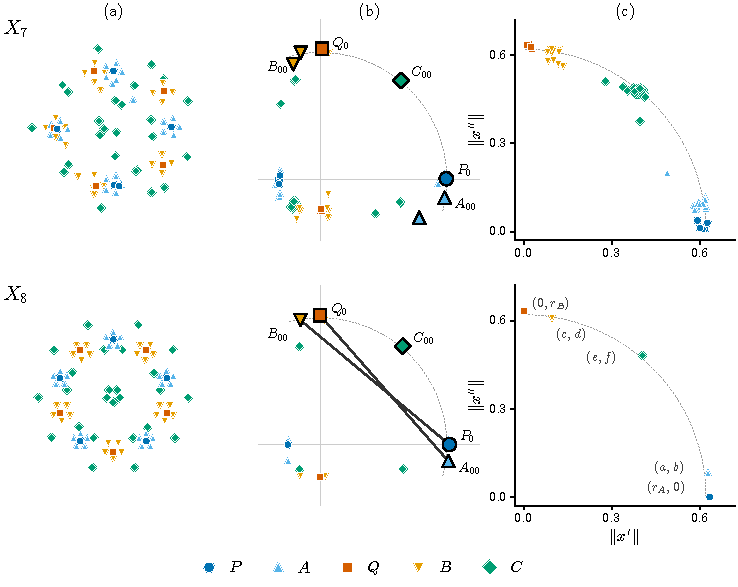
\includegraphics[width=\textwidth]{figs/sets.pdf}
\caption{$X_7$ (top, 84 points in $\R^7$) and $X_8$ (bottom, 85 points in $\R^8$) in three views; $x=(x',x'')\in\R^{m_1}\oplus\R^{m_2}$. Marker: the type of the point (for $X_7$: of the nearest point of $V_7(\theta_7)$). (a)~$x\mapsto\cos\alpha\,\Pi'x'+\sin\alpha\,\Pi''x''$, where $\Pi':\R^{m_1}\to\R^2$ and $\Pi'':\R^{m_2}\to\R^2$ are orthogonal projections that map the $u_i$ and the $v_j$ to regular polygons; $\alpha=50^\circ$ ($n=7$), $45^\circ$ ($n=8$). The $P_i$ form a square ($n=7$) or a pentagon ($n=8$), the $Q_j$ a pentagon; the $A_{ij}$ surround $P_i$, the $B_{ij}$ surround $Q_j$. (b)~$x\mapsto(\langle x',u_0\rangle,\langle x'',v_0\rangle)$, the plane of cell $(0,0)$ (large markers). Lines ($X_8$): the pairs $P_0B_{00}$ and $Q_0A_{00}$, both at distance $\ge s$ (Theorem~\ref{thm:x78}). (c)~$x\mapsto(\|x'\|,\|x''\|)$; in $X_8$ each type is a single point, labelled with its coordinates. Dotted arcs: radius $0.62$; every point of $X_8$ has norm $0.617$ to $0.633$.}
\label{fig:sets}
\end{figure}

\begin{theorem}\label{thm:x78}
\begin{align*}
\frac{\beta_8(X_7)}{\diam X_7}&=\sqrt{\frac{8900856812318928}{10000000213244525}}=0.9434435130\ldots>\sigma_7,\\
\frac{\beta_9(X_8)}{\diam X_8}&=\sqrt{\frac{9023994457279939}{10000000157507010}}=0.9499470677\ldots>\sigma_8.
\end{align*}
\end{theorem}

\begin{proof}
In each fraction the numerator is $10^{16}s^2$ and the denominator $10^{16}D^2$, where $D=\diam X$ and $s$ is the claimed value of $\beta_{n+1}(X)$. By Lemma~\ref{lem:crit} we need three facts: (i)~$G_{\ge s}(X)$ has no proper $(n+1)$-colouring; (ii)~$G_{>s}(X)$ has one; (iii)~the test~\eqref{eq:test}. Table~\ref{tab:cert} lists the checks. (ii) is an explicit colouring, checked edge by edge, and (iii) is integer arithmetic. (i) is checked three ways: by two exhaustive backtracking searches with different symmetry breaking; by a DRAT proof~\cite{WHH14}, a certificate, checked by the program \texttt{drat-trim}, that the Boolean formula ``$G_{\ge s}(X)$ has a proper $(n+1)$-colouring'' is unsatisfiable; and in Lean (\S\ref{sec:lean}). For $X_8$, (i) also follows by hand from Lemma~\ref{lem:colour} (\S\ref{sec:family}).
\end{proof}

\begin{table}[h]
\centering\small
\caption{Certificates for Theorem~\ref{thm:x78}: \href{\repo Riemann/Deep/Gale7/verify.py}{\texttt{verify.py}} (Python standard library, exact integers; search nodes of its two searches), DRAT proofs \href{\repo Riemann/Deep/Gale7/cert7.drat}{\texttt{cert7.drat}}, \href{\repo Riemann/Deep/Gale7/cert8.drat}{\texttt{cert8.drat}}.}
\label{tab:cert}
\begin{tabular}{@{}lrrrrl@{}}
\toprule
 & edges of $G_{\ge s}(X)$ & search nodes & DRAT proof & \texttt{verify.py} & Lean proof of (i)\\
\midrule
$X_7$ & 1765 & 1327; 23097 & 188 KB & 1 s & replay of an 18887-step case split\\
$X_8$ & 2195 & 169807; 801496 & 1.2 MB & 37 s & Lemma~\ref{lem:colour}\\
\bottomrule
\end{tabular}
\end{table}

\section{The family $V_n$ and the colouring lemma}\label{sec:family}

For $5\le n\le 1000$ let $\theta_n$ be row $n$ of \href{\repo Riemann/Deep/Gale7/family_params.txt}{\texttt{family\_params.txt}} (12 decimals, read as exact rationals; $\theta_7,\theta_8$ in Table~\ref{tab:params}). In $V_n(\theta_n)$ the poles $P_i$ are pairwise at distance about $1\approx\diam V_n(\theta_n)$, so a partition into parts of diameter $<1$ puts them in different parts, and likewise the $Q_j$. With $n+1=p+q-1$ parts, some part then contains a $P_i$ and a $Q_j$, which is allowed: $\|P_i-Q_j\|^2=r_A^2+r_B^2\approx 0.8$. The points $A_{ij}$, $B_{ij}$, $C_{ij}$ are placed so that such a part, or another one, gets two points far apart. Table~\ref{tab:H} lists the far pairs that we use; they form the graph $H(p,q)$ (Fig.~\ref{fig:H}).

\begin{table}[h]
\centering\small
\begin{minipage}[c]{0.55\textwidth}\centering
\captionsetup{justification=raggedright,singlelinecheck=false}
\caption{$H(p,q)$: the graph on the vertices $P_i,Q_j,A_{ij},B_{ij},C_{ij}$ ($i\in I$, $j\in J$, $|I|=p$, $|J|=q$). Two vertices are adjacent exactly when the entry for their types holds (---: never).}\label{tab:H}
\setlength{\tabcolsep}{4pt}
\begin{tabular}{@{}lccccc@{}}
\toprule
 & $P_{i'}$ & $Q_{j'}$ & $A_{i'j'}$ & $B_{i'j'}$ & $C_{i'j'}$\\
\midrule
$P_i$ & $i\ne i'$ & --- & $i\ne i'$ & $i=i'$ & $i\ne i'$\\
$Q_j$ & --- & $j\ne j'$ & $j=j'$ & $j\ne j'$ & $j\ne j'$\\
$A_{ij}$ & $i\ne i'$ & $j=j'$ & $i\ne i'$ & --- & $i\ne i'$\\
$B_{ij}$ & $i=i'$ & $j\ne j'$ & --- & $j\ne j'$ & $j\ne j'$\\
$C_{ij}$ & $i\ne i'$ & $j\ne j'$ & $i\ne i'$ & $j\ne j'$ & $i\ne i',\ j\ne j'$\\
\bottomrule
\end{tabular}
\end{minipage}\hfill
\begin{minipage}[c]{0.4\textwidth}\centering
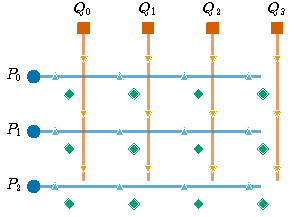
\includegraphics[width=\textwidth]{figs/hgraph.pdf}
\captionof{figure}{$H(3,4)$, vertices only. Blue lines: row blocks $\RB_i=\{P_i\}\cup\{A_{ij}\}_{j}$; orange lines: column blocks $\CB_j=\{Q_j\}\cup\{B_{ij}\}_{i}$; $C_{ij}$ (green) in cell $(i,j)$.}\label{fig:H}
\end{minipage}
\end{table}

\begin{lemma}[colouring lemma]\label{lem:colour}
$\chi(H(p,q))=p+q$ for all $p,q\ge 1$.
\end{lemma}

\begin{proof}
\emph{At most $p+q$.} Colour $P_i$, all $A_{ij}$ and all $C_{ij}$ with colour $i$, and $Q_j$ and all $B_{ij}$ with colour $p+j$; by Table~\ref{tab:H} no two vertices of one colour are adjacent.

\emph{At least $p+q$.} Vertex $C_{ij}$ lies in \emph{row} $i$ and \emph{column} $j$. Let $\RB_i=\{P_i\}\cup\{A_{ij}:j\in J\}$ (row blocks) and $\CB_j=\{Q_j\}\cup\{B_{ij}:i\in I\}$ (column blocks), as in Fig.~\ref{fig:H}. Let $\varphi$ be a proper colouring of $H(p,q)$ with colour set $K$. A colour \emph{meets} a set if some vertex of the set has that colour. Table~\ref{tab:H} gives three facts.
(i)~For $i\ne i'$ every vertex of $\RB_i$ is adjacent to every vertex of $\RB_{i'}$; so a colour meets at most one row block, and likewise at most one column block.
(ii)~$C_{ij}$ is adjacent to every vertex of $\RB_{i'}$ ($i'\ne i$) and of $\CB_{j'}$ ($j'\ne j$); so the colour of $C_{ij}$ meets no row block other than $\RB_i$ and no column block other than $\CB_j$.
(iii)~$C_{ij}$ and $C_{i'j'}$ are adjacent if and only if $i\ne i'$ and $j\ne j'$; so any two $C$-vertices of one colour share a row or a column, and hence all of them lie in one row or in one column.

Split $K$ into $K_1$ (colours that meet a row block but no column block), $K_2$ (a column block but no row block), $K_{12}$ (both) and $K_0$ (neither). A colour in $K_0$ is used only on $C$-vertices; by (iii) choose a row or a column that contains them. Let $I_1$ and $J_1$ be the chosen rows and columns, so $|I_1|+|J_1|\le|K_0|$. Let $I_0$ be the set of rows $i$ such that no colour of $K_1$ meets $\RB_i$, let $J_0$ be the set of columns $j$ such that no colour of $K_2$ meets $\CB_j$, and put $g=|I_0\setminus I_1|$, $h=|J_0\setminus J_1|$.

The rows outside $I_0$ meet distinct colours of $K_1$ by (i), so $|K_1|\ge p-|I_0|\ge p-g-|I_1|$; likewise $|K_2|\ge q-h-|J_1|$. Hence
\begin{equation}\label{eq:count}
|K|=|K_1|+|K_2|+|K_{12}|+|K_0|\ \ge\ p+q-g-h+|K_{12}|.
\end{equation}
For $i\in I_0$ the colour of $P_i$ meets $\RB_i$ and is not in $K_1$, so it is in $K_{12}$; by (i) different rows give different colours, so $|K_{12}|\ge|I_0|\ge g$, and likewise $|K_{12}|\ge h$. For $i\in I_0\setminus I_1$ and $j\in J_0\setminus J_1$ the colour of $C_{ij}$ is in $K_{12}$ and meets $\RB_i$ and $\CB_j$: by (ii) it meets no other blocks; it is not in $K_1$ as $i\in I_0$, not in $K_2$ as $j\in J_0$, and not in $K_0$ as $i\notin I_1$ and $j\notin J_1$. By (i) these $gh$ colours are distinct, so $|K_{12}|\ge gh$.

Now suppose $|K|\le p+q-1$. Then $|K_{12}|\le g+h-1$ by~\eqref{eq:count}. With $|K_{12}|\ge g$ and $|K_{12}|\ge h$ this gives $g,h\ge 1$, and with $|K_{12}|\ge gh$ it gives $(g-1)(h-1)\le 0$, so $g=1$ or $h=1$. Let $g=1$ and $I_0\setminus I_1=\{i^*\}$. Then $|K_{12}|\le h$, so $K_{12}$ consists of the $h$ colours of the $C_{i^*j}$ with $j\in J_0\setminus J_1$, and the colour of $C_{i^*j}$ meets no column block other than $\CB_j$. The colour of $P_{i^*}$ is in $K_{12}$ (as $i^*\in I_0$), so it is the colour of some $C_{i^*j_0}$. The colour of $B_{i^*j_0}$ meets $\CB_{j_0}$ and is not in $K_2$ (as $j_0\in J_0$), so it is in $K_{12}$, hence also the colour of $C_{i^*j_0}$. So $P_{i^*}$ and $B_{i^*j_0}$ have the same colour, but they are adjacent. The case $h=1$ is the same with $Q$, $A$ in place of $P$, $B$.
\end{proof}

\begin{theorem}\label{thm:family}
Let $5\le n\le 1000$. Read each point $P_i,\dots,C_{ij}$ of $V_n(\theta_n)$ as the vertex of $H(p,q)$ with the same name, let $s_n$ be the least distance between two adjacent ones, and let $D_n=\diam V_n(\theta_n)$. Then $\beta_{n+1}(V_n(\theta_n))\ge s_n>\sigma_n D_n$.
\end{theorem}

\begin{proof}
Every edge of $H(p,q)$ joins two points at distance $\ge s_n$, so a proper $(n+1)$-colouring of $G_{\ge s_n}(V_n(\theta_n))$ would give one of $H(p,q)$. As $p+q=n+2$, Lemma~\ref{lem:colour} excludes this, and Lemma~\ref{lem:crit}(a) gives $\beta_{n+1}\ge s_n$. By~\eqref{eq:dist}, $D_n^2$ is the largest of the 36 class values and $s_n^2$ the least of the 17 classes that contain edges of $H(p,q)$; for each $n$, exact rational arithmetic confirms the test~\eqref{eq:test} (\href{\repo Riemann/Deep/Gale7/family.py}{\texttt{family.py}}, 2~s for all 996 rows).
\end{proof}

The gap $s_n/D_n-\sigma_n$ lies between $2.9\cdot10^{-7}$ ($n=1000$) and $1.4\cdot10^{-3}$ ($n=7$); near $n=1000$ it is about $0.29/n^2$. The parameters $\theta_n$ come from a numerical maximization of $s_n/D_n$; any $\theta$ that passes~\eqref{eq:test} works. For $n=3,4$ the best parameters we found give only $s_n/D_n=0.8752<\sigma_3$ and $0.9106<\sigma_4$.

\section{Every dimension $n\ge 3$}\label{sec:all}

\begin{proof}[Proof of Theorem~\ref{thm:main}]
For $n=3,4$ we use our point sets $X_3$ (170 points, \href{\repo Riemann/Deep/Gale/points.txt}{\texttt{Gale/points.txt}}) and $X_4$ (126 points, \href{\repo Riemann/Deep/Gale45/points4.txt}{\texttt{Gale45/points4.txt}}), certified as in Theorem~\ref{thm:x78}; Table~\ref{tab:main} gives the ratios. For $5\le n\le 1000$ we use Theorem~\ref{thm:family}. For $n>1000$, Borsuk's conjecture fails~\cite[Thm.~1]{Hi02}: there is a bounded $S\subset\R^n$ with at least two points such that every partition of $S$ into $n+1$ parts has a part of diameter $\diam S$. If $\beta_{n+1}(S)\le\sigma_n\diam S$, then, as $\sigma_n<1$, some partition of $S$ into $n+1$ parts would have all parts of diameter less than $\diam S$. So $S$ is a counterexample.
\end{proof}

The same argument shows that every counterexample to Borsuk's conjecture is a counterexample to Gale's.

\section{Lean formalization}\label{sec:lean}

All results are formalized in Lean~4 (v4.35.0-rc2) with Mathlib~\cite{dMU21,mC20}, on $\R^n$ as \texttt{EuclideanSpace} with Mathlib's diameter (Table~\ref{tab:lean}). There, \texttt{GaleConjecture n} states that $\R^n$ has no counterexample. The proofs contain no \texttt{sorry} and use only the axioms \texttt{propext}, \texttt{Classical.choice} and \texttt{Quot.sound}; the finite checks run in the Lean kernel (\texttt{decide +kernel}). Two cited facts enter as hypotheses: Hinrichs's theorem~\cite{Hi02}, used only for $n>1000$, and $\beta_{n+1}(B^n)\le\sigma_n$~\cite{Vo26}, used only to pass from counterexamples to Gale's conjecture itself. \href{\repo papers/02_gale-fails-every-dimension/PROOF.md}{\texttt{PROOF.md}} maps every step of this paper to Lean.

\begin{table}[h]
\centering\small
\captionsetup{justification=raggedright,singlelinecheck=false}
\caption{Lean names (links). Files are in \href{\repo Riemann/Deep/LeanGale}{\texttt{Riemann/Deep/LeanGale}}, except \texttt{Lemma.lean} (in \href{\repo Riemann/Deep/Gale7/Lean}{\texttt{Riemann/Deep/Gale7/Lean}}).}
\label{tab:lean}
\begin{tabular}{@{}lll@{}}
\toprule
statement & Lean & file\\
\midrule
$\beta_k$; no counterexample & \lean{beta}{Riemann/Deep/LeanGale/Gale.lean\#L25-L28}; \lean{GaleConjecture}{Riemann/Deep/LeanGale/Gale.lean\#L30-L33} & \texttt{Gale.lean}\\
Lemma~\ref{lem:crit}(a) with~\eqref{eq:test} & \lean{sigma\_mul\_diam\_lt\_beta}{Riemann/Deep/LeanGale/Gale.lean\#L137-L155} & \texttt{Gale.lean}\\
Theorem~\ref{thm:x78} & \lean{claim1\_n7}{Riemann/Deep/LeanGale/Main.lean\#L93-L124}, \lean{claim1\_n8}{Riemann/Deep/LeanGale/Main.lean\#L137-L156} & \texttt{Main.lean}\\
Lemma~\ref{lem:colour} & \lean{card\_le}{Riemann/Deep/Gale7/Lean/Lemma.lean\#L435-L460} & \texttt{Lemma.lean}\\
Theorem~\ref{thm:family} & \lean{claim2}{Riemann/Deep/LeanGale/Main.lean\#L202-L215} & \texttt{Main.lean}\\
Theorem~\ref{thm:main}, $n\le 1000$ & \lean{gale\_fails\_le\_1000}{Riemann/Deep/LeanGale/Main.lean\#L227-L236} & \texttt{Main.lean}\\
Theorem~\ref{thm:main}, all $n\ge 3$ & \lean{gale\_fails}{Riemann/Deep/LeanGale/Main.lean\#L266-L273}, \lean{gale\_ball\_fails}{Riemann/Deep/LeanGale/Main.lean\#L283-L289} & \texttt{Main.lean}\\
\bottomrule
\end{tabular}
\end{table}

\begin{thebibliography}{99}\small\raggedright
\bibitem{Bo33} K.~Borsuk, Drei S\"atze \"uber die $n$-dimensionale euklidische Sph\"are, \emph{Fund.\ Math.}\ 20 (1933) 177--190, doi:10.4064/fm-20-1-177-190.
\bibitem{dMU21} L.~de~Moura, S.~Ullrich, The Lean~4 theorem prover and programming language, \emph{CADE-28}, LNCS 12699 (2021) 625--635, doi:10.1007/978-3-030-79876-5\_37.
\bibitem{Ga53} D.~Gale, On inscribing $n$-dimensional sets in a regular $n$-simplex, \emph{Proc.\ Amer.\ Math.\ Soc.}\ 4 (1953) 222--225, doi:10.1090/S0002-9939-1953-0053534-7.
\bibitem{Hi02} A.~Hinrichs, Spherical codes and Borsuk's conjecture, \emph{Discrete Math.}\ 243 (2002) 253--256, doi:10.1016/S0012-365X(01)00202-3.
\bibitem{JB14} T.~Jenrich, A.~E.~Brouwer, A 64-dimensional counterexample to Borsuk's conjecture, \emph{Electron.\ J.\ Combin.}\ 21(4) (2014) P4.29, doi:10.37236/4069.
\bibitem{KK93} J.~Kahn, G.~Kalai, A counterexample to Borsuk's conjecture, \emph{Bull.\ Amer.\ Math.\ Soc.}\ 29 (1993) 60--62, doi:10.1090/S0273-0979-1993-00398-7.
\bibitem{mC20} The mathlib Community, The Lean mathematical library, \emph{CPP 2020}, 367--381, doi:10.1145/3372885.3373824.
\bibitem{OAI26} OpenAI, A nine-dimensional counterexample to Borsuk's covering assertion, preprint (2026), \url{https://github.com/openai/math}.
\bibitem{Vo26} V.~Voronov, A counterexample to Gale's conjecture in $\R^3$, arXiv:2610.28828 (2026).
\bibitem{WHH14} N.~Wetzler, M.~J.~H.~Heule, W.~A.~Hunt~Jr., DRAT-trim: efficient checking and trimming using expressive clausal proofs, \emph{SAT 2014}, LNCS (2014) 422--429, doi:10.1007/978-3-319-09284-3\_31.
\end{thebibliography}

\end{document}
